\section{Steering Large Language Models using APE}
% This section examines how APE can guide LLMs to desired behaviors. We investigate from three perspectives: zero-shot performance, few-shot in-context learning performance, and truthfulness.

\subsection{Instruction Induction}\label{sec:inst_induct}
We assess the effectiveness of \algname~to steer LLMs by evaluating the zero-shot performance of another LLM following the selected instruction on 24 instruction induction tasks proposed in \citet{honovich2022instruction}. 
% The tasks span many facets of language understanding, from simple phrase structure to similarity and causality identification. We refer the reader to Appendix A of \citet{honovich2022instruction} for detailed descriptions of each task. 
 For each task, we sample five input-output pairs from the training data and select the best instruction using algorithm \ref{alg:ape}. Then, we evaluate the quality of the instruction by executing the instruction on InstructGPT (175B)\footnote{We use the  \textit{text-davinci-002} via the OpenAI API (\url{https://beta.openai.com/}). Though not stated explicitly in the API, we assume the models are those reported by \citet{ouyang2022training}.}. We repeat our experiments with different random seeds five times to report the mean and standard deviation of the best-performing result in each seed. Moreover, we examine various properties of \algname, such as scalability to model sizes, quality of the initial proposal, the effectiveness of the selection, and application on few-shot learning. For conciseness, we defer more experimental results and implementation details in Appendix \ref{app:add_res} and \ref{app:imp_details}.

% and report the best overall performance in Appendix Figure \ref{fig:app-zero-shot-best}. The exact templates for our experiments can be found in Appendix Table \ref{table:raw_templates}.

\begin{figure}[tb]
    \vspace{-0.25in}
  \centering
  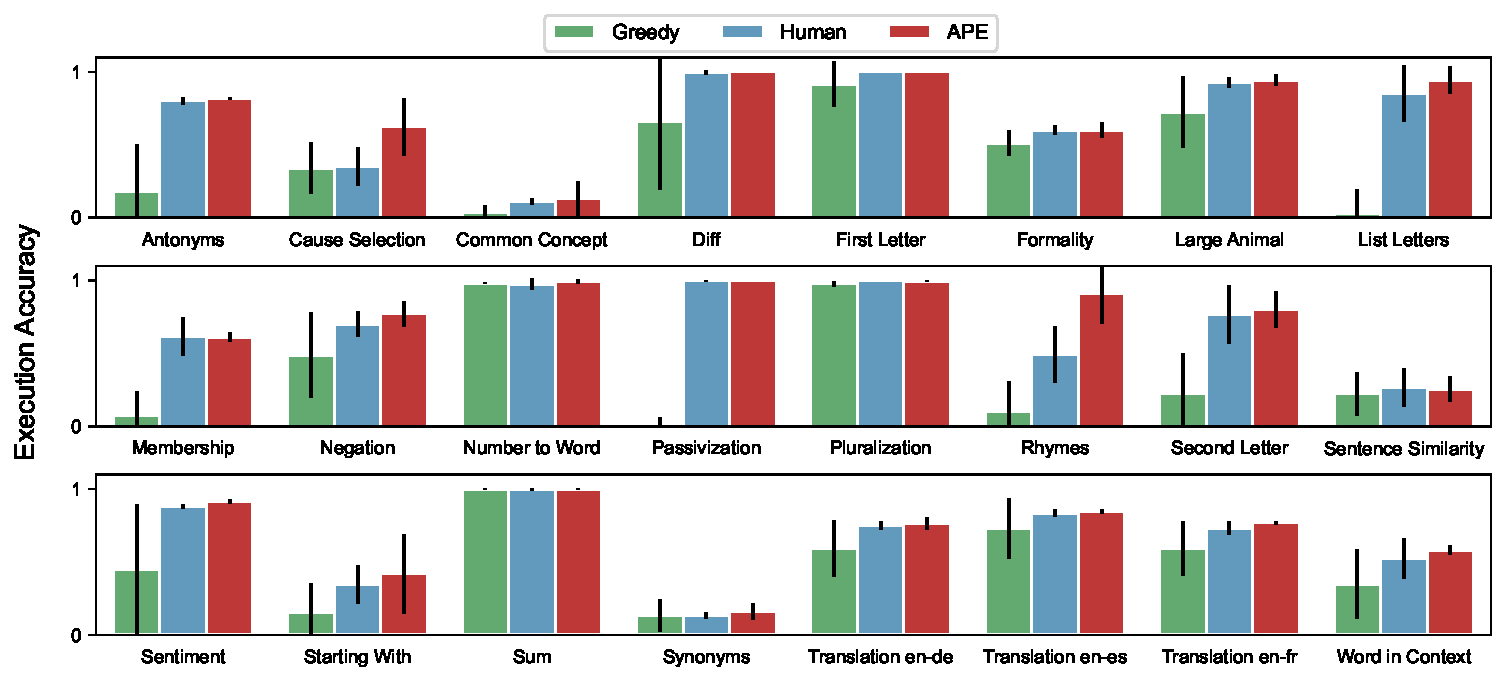
\includegraphics[width=0.95\linewidth]{figures/main/exec_acc_zero_shot.pdf}
  \caption{Zero-shot test accuracy on 24 Instruction Induction tasks. \algname~achieves human-level performance on 19 out of 24 tasks. See best performing instruction performance in Figure \ref{fig:app-zero-shot-best}.}\label{fig:main-zero-shot}
\end{figure}

\paragraph{Zero-shot Learning}
We compare our method against two baselines: human prompt engineers (Human)\footnote{\mbox{We use the gold annotations from \citet{honovich2022instruction}, which were manually verified for correctness.}} and the model-generated instruction algorithm proposed by \citet{honovich2022instruction}. This algorithm can be thought of as a greedy version of \algname, without a search and selection process; thus, we refer to it as ``Greedy''. Figure \ref{fig:main-zero-shot} shows the zero-shot performance of InstructGPT using human instructions and model generated instructions. Our algorithm outperforms ``Greedy'' on every task and achieves equal or better than human performance on 24 of 24 tasks. Moreover, the Interquartile Mean (IQM) \citep{agarwal2021deep} across all 24 tasks in Figure \ref{fig:highlight} suggests that \algname~with InstructGPT outperforms human-engineered prompts, obtaining an IQM of 0.810 vs humans' 0.749. We summarize the instruction selected by \algname~for each task in Appendix Table \ref{table:best_instructions_all}.

\subsection{TruthfulQA}\label{subsec:truthfulqa}
We apply our method on TruthfulQA \citep{lin2022truthfulqa} to see how \algname-generated instructions can steer an LLM to generate answers with different styles, and study the trade-off between truthfulness and informativeness. Borrowing the metrics from the original paper, we use \algname~to the learn instructions that maximize three metrics: truthfulness (\% True), informativeness (\% Info), and a combination of both (\%True + \%Info). \citet{lin2022truthfulqa} used human evaluation to assess the model performance, but they found their automated metrics align with human prediction over 90\% of the time. In our experiments, we rely on their fine-tuned GPT-judge and GPT-info to evaluate the scores. 

\paragraph{Prompt Engineering in TruthfulQA} We want to stress that the TruthfulQA dataset is intended to test pretrained models in zero-shot settings. Our results are not in any way compatible with the original benchmarks. Because we have optimized the instructions using a small portion of the question and answer pairs as training demonstrations, our results are not ``true few-shot learning''~\citep{perez2021true}. We randomly sampled 100 out of 817 questions for the actual experiments to form training demonstrations $\trainingData$. To sample the proposal set $\proposal$, we ask a ``reverse'' model to generate instructions based on 6 randomly chosen demonstration pairs, similar to our previous experiments. Unlike in Instruction Induction, in TruthfulQA, we aim to find a single best instruction prompt that works well across all 38 categories of questions spanning health, law, politics, and fiction. It is worth noting all our generated instructions are very generic, 
% e.g., ``You will be asked a series of questions. For each question, you must either answer the question or decline to answer, in which case you must state that you have no comment'', 
and do not contain any examples from the dataset. We provide a list of top 10 instructions selected by APE using different metrics in Table \ref{table:truthfulqa_true}, \ref{table:truthfulqa_info}, \ref{table:truthfulqa_both}.

\paragraph{Truthfulness vs Informativeness Trade-off}
We found that \algname~outperforms the human-engineered prompt with only 200 candidates proposed by InstructGPT (175B), as seen in Figure~\ref{fig:truthfulqa}. We compared our generated prompt with the ``help'' prompt from \citet{lin2022truthfulqa}.
The training and test performance are shown in Figure~\ref{fig:truthfulqa}(a)-(b). We found that choosing the top 10 of 200 candidates on the training set generalizes well to the test set. We report the average performance across the top 10 instructions for the three metrics.
This result by itself is not surprising as the human baseline is not carefully chosen, as pointed out by \citet{askell2021general}. However, we found that the instructions discovered by \algname~can achieve very high truthfulness with answers such as ``No comment'' but these answers provide little information. We used our top candidates to further investigate the trade-off between truthfulness and informativeness. We visualize the top 10 proposed samples across the three metrics on the truthfulness-informative plots shown in Figure~\ref{fig:truthfulqa}(c) and Figure~\ref{fig:truthfulqa}(d). While \algname~achieves over 40\% accuracy in providing both true and informative answers (v.s. 30\% by the ``help'' prompt from humans), the instructions discovered tend to target the two ends of this \%true-\%info Pareto frontier. 

\begin{figure}
  \vspace{-0.25in}
  \centering
%   \fbox{\rule[-.5cm]{0cm}{4cm} \rule[-.5cm]{4cm}{0cm}}
\begin{subfigure}[b]{0.245\textwidth}
  \captionsetup{justification=centering}
  \hfill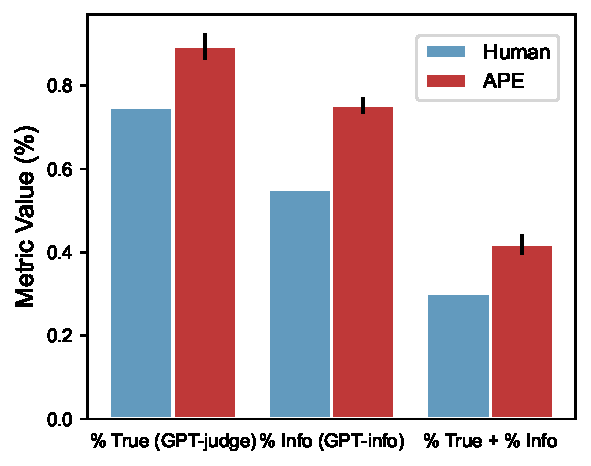
\includegraphics[width=1.0\linewidth]{figures/main/truthfulqa_top10_train.pdf}
  \caption{Average performance Train}
\end{subfigure}
\begin{subfigure}[b]{0.245\textwidth}
  \captionsetup{justification=centering}
  \hfill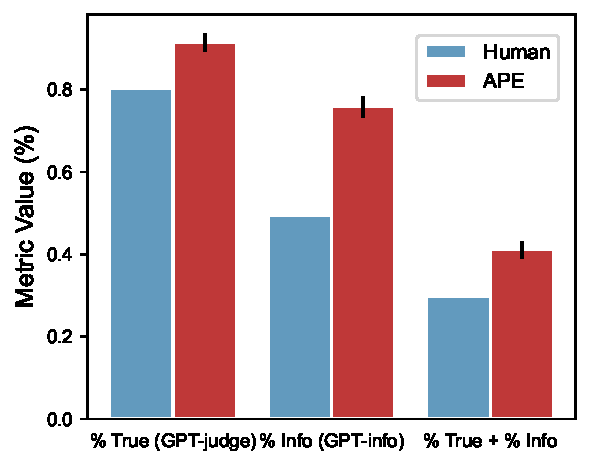
\includegraphics[width=1.0\linewidth]{figures/main/truthfulqa_top10_test.pdf}
  \caption{Average performance Test}
\end{subfigure}
\begin{subfigure}[b]{0.245\textwidth}
  \captionsetup{justification=centering}
  \hfill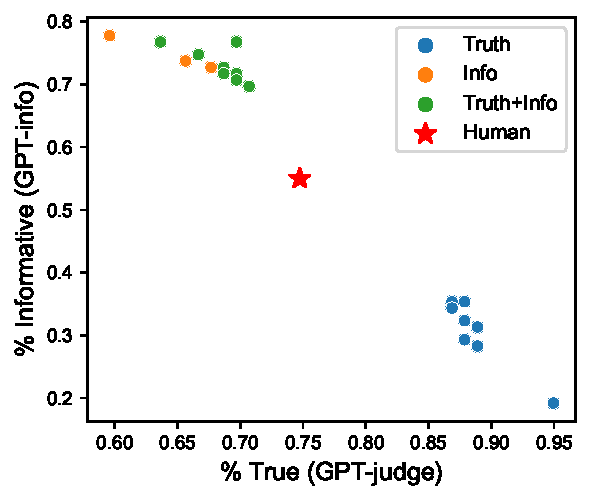
\includegraphics[width=1.0\linewidth]{figures/main/truthfulqa_scatter_train.pdf}
  \vspace{-1.6em}
  \caption{\%True-\%Info trade-off Training}
\end{subfigure}
\begin{subfigure}[b]{0.245\textwidth}
  \captionsetup{justification=centering}
  \hfill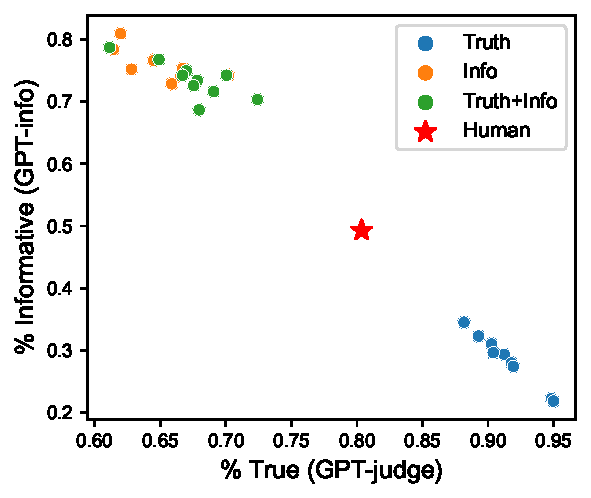
\includegraphics[width=1.0\linewidth]{figures/main/truthfulqa_scatter_test.pdf}
  \vspace{-1.6em}
  \caption{\%True-\%Info trade-off Test}
\end{subfigure} \vspace{-0.15in}
  \caption{Comparison of \algname~and ``help'' (human) prompt on the TruthfulQA task. (a) Percentage of answers that were either true (\% True), informative (\% Info), or both (\% True + \% Info) on the 100 training examples. (b) Same data on the 717 test examples. (c) \%True-\%Info frontier computed on training data with top 10 instructions from each metric. (d) \%True-\%Info frontier on the test data. }\label{fig:truthfulqa}
\end{figure}